%%% 特別研究報告書サンプル
\documentclass[dvipdfmx]{ampbt}

%%% クラスオプション:
%%% chapter:   \chapterコマンドを使用可能にする(jsbook (report) を使う).
%%% その他 jsclasses に指定可能なオプションが指定できます(そのまま渡される).

%%% 題目 %%%%%%%%%%%%%%%%%%%%%%%%%%%%%%%%%%%%%%%%%%%%%%%%%%%%%%%%%%%%%%%%%%%%%%%%
\title{境界積分方程式法による音場の}     % 題目1行目
      {数値解析と移動する受音点における}      % 題目2行目
      {リアルタイム可聴化について}                % 題目3行目
%%% 指導教員 %%%%%%%%%%%%%%%%%%%%%%%%%%%%%%%%%%%%%%%%%%%%%%%%%%%%%%%%%%%%%%%%%%%%
\supervisors{吉川仁}{准教授}    % 指導教員1人目 {氏名}{職名}
            {}{}    % 指導教員2人目 {氏名}{職名}
            {}{}                % 指導教員3人目 {氏名}{職名}
%%% 入学年月 %%%%%%%%%%%%%%%%%%%%%%%%%%%%%%%%%%%%%%%%%%%%%%%%%%%%%%%%%%%%%%%%%%%%
\entrancedate{26}{4}            % {年(平成)}{月}
%%% 著者氏名 %%%%%%%%%%%%%%%%%%%%%%%%%%%%%%%%%%%%%%%%%%%%%%%%%%%%%%%%%%%%%%%%%%%%
\author{石床}{竜一}             % {姓}{名}
%%% 提出日 %%%%%%%%%%%%%%%%%%%%%%%%%%%%%%%%%%%%%%%%%%%%%%%%%%%%%%%%%%%%%%%%%%%%%%
\submissiondate{30}{1}{26}      % {年(平成)}{月}{日}
%%% 背表紙の出力枚数 %%%%%%%%%%%%%%%%%%%%%%%%%%%%%%%%%%%%%%%%%%%%%%%%%%%%%%%%%%%%
\def\numberofspines{1}
%%% 摘要 %%%%%%%%%%%%%%%%%%%%%%%%%%%%%%%%%%%%%%%%%%%%%%%%%%%%%%%%%%%%%%%%%%%%%%%%
\abstract{%
  本研究では波動方程式に支配される,
  散乱体の存在する音場の数値解析を行った.
  受音点の移動による波形の変化が観測できたが,
  計算時間によるリアルタイム可聴化は実現できなかった.
}
%%% パッケージの読み込みや自分用のマクロの定義 %%%%%%%%%%%%%%%%%%%%%%%%%%%%%%%%%%
\usepackage{amsmath,amssymb}
\usepackage{here}
\usepackage{bm}
\newcommand{\rme}{\mathrm{e}}
\def\bi#1{\mbox{\boldmath$#1$}}
\def\shiki#1{式{(\ref{#1})}}
\def\zu#1{{図\ref{#1}}}
\def\traction#1{{\rm T}#1}
\newcommand{\abs}[1]{|#1|}
\def\vector#1{\mbox{\boldmath $#1$}}

%%% 出力の制御 %%%%%%%%%%%%%%%%%%%%%%%%%%%%%%%%%%%%%%%%%%%%%%%%%%%%%%%%%%%%%%%%%%

%%% 本文を出力しない場合,次の行のコメントを外して下さい.
%% \outputbodyfalse

%%% 末尾に表紙,背表紙を出力しない場合,次の行のコメントを外して下さい.
%% \outputcoverfalse

%%% 末尾に提出用摘要を出力しない場合,次の行のコメントを外して下さい.
%% \outputabstractforsubmissionfalse

%%% ampbt.cls では表紙等の作成のために geometry パッケージを使用しているため,本文
%%% のレイアウトを変えるために \usepackage[...]{geometry} とすると Option clash が
%%% 発生します.何らかの理由で本文のレイアウトを変更したい場合は \geometry{...} を
%%% 使用して下さい.
%%% また,jsclasses を使用しているため,例えば 3cm を指定したい場合は 3truecm と書
%%% く必要があります.
%% \geometry{hmargin=3truecm,vmargin=2truecm}

\begin{document}
\ifoutputbody
%%% 中表紙,摘要,目次 %%%%%%%%%%%%%%%%%%%%%%%%%%%%%%%%%%%%%%%%%%%%%%%%%%%%%%%%%%
\makeinsidecover                % 中表紙
\makeabstract                   % 摘要
\maketoc                        % 目次
\setcounter{page}{1}            % 本文のページ番号を1から始める
%%% 本文 %%%%%%%%%%%%%%%%%%%%%%%%%%%%%%%%%%%%%%%%%%%%%%%%%%%%%%%%%%%%%%%%%%%%%%%%
\section{序論}

% 生活音や音楽また騒音に至るまで,音はいろいろな場所で聞くことができる.
% コンサートホール,工事現場,カラオケなど音を扱うあるいは発生するような場は音響理論にもとづいて設計されているが,
% 音響のシミュレーションが可能であれば,実際に壁を設営する前にその壁の影響で
% どのように音が変化するかを提示することができるため,コスト削減等に寄与できると考えられる.
% シミュレーションで音場を取り扱う際には幾何音響理論と波動音響理論が一般的である.
% 幾何音響理論では音を波動としてはとらえず,エネルギーの伝搬を考えるため,リアルタイム性が要求されるような場で一般的に用いられる.


生活音や音楽また騒音に至るまで,音はいろいろな場所で聞くことが可能だが,
散乱体が存在する場合,音は散乱体の影響で変化すると考えられる.
コンサートホール,工事現場,カラオケなど音を扱う,あるいは発生する場において,
音響のシミュレーションで音がどのように変化するかを確認することができれば,
実際に壁を設営するか否かの指標になり,建設コスト削減や騒音被害等に寄与できると考えられる.
このとき視覚,聴覚的な情報があり,どのような状況で音が変化したのかがわかりやすくなるはずである.
音の変化を聴覚的,視覚的かつリアルタイムに観測できるようなシステムを作成し,
本論文では,散乱体の存在する3次元空間での音のリアルタイム可聴化を目標とする.
先行研究では解析手法にリアルタイム性が要求されるような場で一般的に用いられる幾何音響手法を用いていたが,
ここでは境界値を事前に計算しておくことで,
メモリの節約や高速化が見込める境界要素法を用いて計算を行うこととした.
本論文の構成は次の通りである.
まず,第 2 章で 対象とする問題の時間域境界積分方程式による音場解析について述べる.
第 3 章では第 2 章で導いた積分表現に適用した近似について述べる.第 4 章で近似の精度とその近似を用いた実際の計算を述べる.
第 5 章で結論を述べる.


\section{時間域境界積分方程式による音場解析}
\label{2章}
\subsection{対象とする問題}
\label{q}
ある閉じた3次元領域の外部領域$D$における,位置$\bm{x}$,時刻$t$での音圧$u(\bm{x},t)$について
次の初期値境界値問題を考える.
\begin{align}
&\ddot{u}(\bm{x},t)-c^2 u_{,ii}(\bm{x},t)=0,\  \bm{x} \in D,\ t>0 \\
&u(\bm{x},0)=0,\  \vector{x} \in D \\
&\dot{u}(\bm{x},0)=0,\  \vector{x} \in D \\
\label{eq:u_y}
&u(\vector{x},t)=\bar{u}(\bm{x},t),\  \vector{x}\  \mbox{on} \ S_D,\ t>0 \\
\label{eq:q_y}
&\frac{\partial{u}}{\partial{n}} (\bm{x},t)=\bar{q}(\bm{x},t),\  \bm{x}\  \mbox{on} \ S_N,\ t>0 \\
&u(\bm{x},t) \to u^{\mbox{in}}(\bm{x},t),\ |\vector{x}| \to \infty
\end{align}
ここに,$u^{\mbox{in}}(\bm{x},t)$は入射波を$\bar{u}(\bm{x},t)$,$\bar{q}(\bm{x},t)$は既知関数である.また,$(\ )_{,i}$は$\dfrac{\partial{}}{\partial{x_i}}$,

$(\dot{\ })$は$\dfrac{\partial{}}{\partial{t}}$,
$\dfrac{\partial{}}{\partial{n}}$は法線微分で$n_i(\bm{x}) \dfrac{\partial{}}{\partial{x_i}}$,
$n(\bm{x})$は境界上の点$x$における領域の外向き単位法線ベクトル,
$S$は領域$D$の境界で$S=S_D \cup S_N$,
$c$は波速である.

\subsection{解の積分表現}
初期値境界値問題の解は,3次元波動方程式の基本解
\begin{align}
&\Gamma(\bm{x},t) = \displaystyle \frac{\delta(t-\dfrac{|\vector{x}|}{c})}{4\pi|\vector{x}|}
\end{align}
を用いて
\begin{equation}
  \label{eq:境界積分方程式}
u(\bm{x},t) = u^{\mbox{in}}(\vector{x},t) + \int_S\!\!\int_0^t \Gamma(\bm{x}-\vector{y},t-s) \frac{\partial u}{\partial n}(\vector{y},s) - \int_S\!\!\int_0^t \frac{\partial \Gamma}{\partial n}(\bm{x}-y,t-s) u(\vector{y},s) ds dS
\end{equation}
と表すことができる.
ここに$\delta(t)$はDiracのデルタ関数である.

境界条件(式(\ref{eq:u_y})、(\ref{eq:q_y}))より、$S_D$上の$u(\vector{x},t)$と$S_N$上の$\frac{\partial u}{\partial n}(\vector{x},t)$は与えられているが、
$S_N$上の$u(\vector{x},t)$、$S_0$上の$\dfrac{\partial u}{\partial n}(\vector{x},t)$は未知である。
これらの境界量を求めるために、$\vector{x} \in D$を境界$S$に極限移行し、次の境界積分方程式を得る。
\begin{eqnarray}
  \label{eq:境界を求める}
\frac{1}{2} u(\vector{x},t) &=& u^{\rm{in}}(\vector{x},t) + \int_S \int_0^t \Gamma (\vector{x}-\vector{y},t-s) \frac{\partial u}{\partial n}(\vector{y},s) ds dS \nonumber \\
                                               &-& \int_S \int_0^t \frac{\partial \Gamma}{\partial n_y} (\vector{x}-\vector{y},t-s) u(\vector{y},s) ds dS \quad, \vector{x} \in S , t > 0
\end{eqnarray}
まず、式(\ref{eq:境界を求める})を$u(\vector{x},t) , \vector{x} \in S_N$,$\dfrac{\partial u}{\partial n}(\vector{x},t) , \vector{x} \in S_0$について解く。\\
次に、得られた境界量を用いて式(7)により領域$D$の内点での解$u(\vector{x},t)$を得る。

\subsection{時間域境界積分方程式法}
境界積分方程式(\ref{eq:境界を求める})を数値的に解くために,境界$S$を境界要素$S_j
, j=1, \cdots ,N$に分割し,さらに境界量$\displaystyle
u(\bi{x},t),\frac{\partial u}{\partial n}(\bi{x},t)$を空間内挿関数
${M_S}^j(\bi{x})$と時間内挿関数${M_T}^m(t)$を用いて離散化する.
%
\begin{align}
&  u(\bi{x},t) \simeq \sum_{m=1}^{N_T} \sum_{j=1}^{N} u(\vector{p}^j,
  m\Delta t ) {M_S}^j(\bi{x}){M_T}^m(t),\\
&   \frac{\partial u}{\partial n}(\bi{x},t) \simeq \sum_{m=1}^{N_T} \sum_{j=1}^{N} \frac{\partial u}{\partial n}(\bi{p}^j,
  m\Delta t ) {M_S}^j(\bi{x}){M_T}^m(t),
\end{align}
ここに,点$\vector{p}^j$は境界要素$S_j$の代表点で、 $\Delta t$は時間
増分、$N_T$は時間ステップ数である.このとき,ある時刻$t=n\Delta t,\ n = 1,
\cdots,N_T$における離散化された境界積分方程式は次式で得られる..
\begin{align}
  \label{eq:uのシグマ}
&  -\bi{u}_n^{\rm{in}} = \sum_{m=1}^n
  \bi{U}_{n-m+1}{\bi{q}}_m -
  \sum_{m=1}^n\bi{W}_{n-m+1}\bi{u}_m,
\end{align}
%
\begin{align}
 & \{\bi{u}_n^{\rm{in}}\}_i := u^{\rm{in}}(\bi{p}^i,n\Delta
  t),\\
 & \{\bi{u}_m\}_i := u(\bi{p}^i,m\Delta t ),\\
 & \{ {\bi{q}}_m \}_i := \frac{\partial u}{\partial n}(\bi{p}^i,m\Delta t),\\
 & \{\bi{U}_{n-m+1}\}_{ij}  := \int_{S} \int^{\infty}_{-\infty}
  \Gamma(\bi{p}^i - \bi{y},n\Delta t
  - s){M_S}^j(\bi{y}){M_T}^m(s)dsdS,\label{1jyuso}\\
 & \{\bi{W}_{n-m+1}\}_{ij}  := \int_{S} \int^{\infty}_{-\infty}
  \frac{\partial \Gamma}{\partial n_{y}}(\bi{p}^i - \bi{y},n\Delta t
  - s){M_S}^j(\bi{y}){M_T}^m(s)dsdS. \label{2jyuso}
\end{align}
この代数方程式(\ref{eq:uのシグマ})を各時間ステップにおいて逐次的に解く.

式(\ref{eq:uのシグマ})を解き、境界量$\vector{u}_m ,\vector{q}_m ,m=1,\cdots,N_T$が得られたならば、領域$D$内の任意の点$\vector{x}$での時刻$n \Delta t$での値が次式で得られる.
\begin{eqnarray}
  \label{{eq:18}}
u(\vector{x},n \Delta t) &=& u^{\rm{in}}(\vector{x},n \Delta t) \nonumber \\
                                         &+& \sum^{n}_{m=1} \sum^{N}_{j=1} \left\{ \int_{S} \int_{-\infty}^{\infty} \Gamma(\vector{x}-\vector{y},n \Delta t - s)M^{j}_{S}(\vector{y})
                                         M^{m}_{T}(s) ds dS \right\} \left\{ \vector{q}_{m} \right\}_{j} \nonumber \\
                                         &-& \sum^{n}_{m=1} \sum^{N}_{j=1} \left\{ \int_{S} \int_{-\infty}^{\infty} \frac{\partial \Gamma}{\partial n_y}(\vector{x}-\vector{y},n \Delta t - s)
                                         M^{j}_{S}(\vector{y}) M^{m}_{T}(s) ds dS \right\} \left\{ \vector{u}_{m} \right\}_{j}
\end{eqnarray}

\section{移動する受音点での音圧の計算}
\label{3章}
\subsection{境界積分方程式の近似}
\label{kinji}
本研究では,VR空間内を移動する人が聴く音を作り出すことを目標とし,音圧をリアルタイムで計算することを目的とする.移動する受音点の各時刻での
内点計算(式(\ref{eq:18}))の計算時間短縮のために次の近似を考える.






\begin{eqnarray}
&&\int_S\int_0^{n\Delta t}\frac{\delta (n\Delta t-s-\frac{|\vector{x}-\vector{y}|}{c})}{4\pi |\vector{x}-\vector{y}|} \frac{\partial u}{\partial n}(\vector{y},s)dsdS  \nonumber \\
&\simeq&\sum_{j=1}^N \int_{S_j} \frac{1}{4\pi |\vector{x}-\vector{y}|} \frac{\partial u}{\partial n}(\vector{y},n\Delta t-\frac{|\vector{x}-\vector{y}|}{c}) H(n\Delta t-\frac{|\vector{x}-\vector{y}|}{c})dS \nonumber \\
&\simeq& \sum_{j=1}^N \frac{1}{4\pi |\vector{x}-\vector{p}^j|}  \frac{\partial u}{\partial n}(\vector{p}^j,n\Delta t-\frac{|\vector{x}-\vector{p}^j|}{c})H(n\Delta t-\frac{|\vector{x}-\vector{p}^j|}{c})|S_j|
\end{eqnarray}
ここに,$\frac{\partial u}{\partial n}\left(\vector{p}^j,n\Delta t-\frac{|\vector{x}-\vector{p}^j|}{c} \right)$は時刻$n\Delta t-\mathrm{int}\left( \frac{|\vector{x}-\vector{p}^j|}{c\Delta t} \right)\Delta t$のと時刻
$(n+1)\Delta t-\mathrm{int}\left( \frac{|\vector{x}-\vector{p}^j|}{c\Delta t}\right)\Delta t$との$\frac{\partial u}{\partial n}$の値を線形補間することで求める.
また$H(t)$はヘビサイド関数であり,$|S_j|$は境界要素$S_j$の面積である.

式(8)右辺第3項について

\begin{eqnarray}
\lefteqn{\int_{S} \int_{0}^{n \Delta t} \frac{\partial }{\partial n_{y}} \left( \frac{\delta \left(n \Delta t -s - \frac{|\vector{x}-\vector{y}|}{c}\right)}{4 \pi |\vector{x} - \vector{y}|} \right) u(\vector{y},s) ds dS }  \nonumber \\
& \simeq & \sum^{N}_{j=1} -n_{i}(\vector{P}^{j}) \frac{\partial }{\partial x_i} \int_{S_j}
 \int_{0}^{n \Delta t} \frac{\delta \left(n \Delta t -s - \frac{|\vector{x}-\vector{y}|}{c}\right)}{4 \pi |\vector{x} - \vector{y}|} u(\vector{y},s) ds dS \nonumber \\
& \simeq & \sum^{N}_{j=1} -n_{i}(\vector{P}^{j}) \frac{\partial }{\partial x_i} \int_{S_j}
  \int_{0}^{n \Delta t} \frac{\delta \left(n \Delta t -s - \frac{|\vector{x}-\vector{y}|}{c}\right)}{4 \pi |\vector{x} - \vector{y}|} \sum^{n}_{m=1} M_{T}^{m}(s) u(\vector{y},m \Delta t) ds dS \nonumber \\
& \simeq & \sum^{N}_{j=1} -n_{i}(\vector{P}^{j}) \frac{\partial }{\partial x_i} \int_{S_j}
    \sum^{n}_{m=1} \frac{M_{T}^{m} \left(n \Delta t - \frac{|\vector{x}-\vector{y}|}{c}\right)}{4 \pi |\vector{x} - \vector{y}|}  u(\vector{y},m \Delta t) H \left( n \Delta t - \frac{|\vector{x}-\vector{y}|}{c} \right) dS \nonumber \\
& \simeq & \sum^{N}_{j=1} -n_{i}(\vector{P}^{j}) |S_j| \sum^{n}_{m=1} \frac{\partial }{\partial x_i}
\left\{ \frac{M_{T}^{m} \left(n \Delta t - \frac{|\vector{x}-\vector{P}^{j}|}{c}\right)}
    {4 \pi |\vector{x} - \vector{P}^{j}|}  u(\vector{y},m \Delta t) \right\} H \left( n \Delta t - \frac{|\vector{x}-\vector{P}^{j}|}{c} \right) dS \nonumber
\end{eqnarray}

今回の解析では、時間内挿関数$M_T^{m}(t)$として$2 \Delta t$のサポートを持つ区分線形関数を用いる。
このとき、図!!!!まだない!!!!!のように特定の時刻$n \Delta t - \frac{|\vector{x}-\vector{P}^{j}|}{c}$
において非ゼロの値を返す$M_{T}^{m}(t)$は2つのみであるから、式(20)の添字$m$についての総和は2項の足し算に過ぎない。



決められた時間内に特定の処理を終えなければならない制約ができる.そのため式(\ref{eq:境界積分方程式})を近似することを考える.\par
以降この式を用いて,移動する内点$\vector{x}$の各時間ステップ毎の音圧を計算する.



\section{数値結果}
\subsection{精度検証}
%\label{境界値の取得}
\ref{kinji}節で示した近似式の精度を検証するために次のような境界値を持つ3次元の音場を考える.各辺がデカルト座標軸に平行な中心$\bm{x}^{\rm{s}} =(0.5,0.5,0.5)$,辺の長さ1の立方体の外部領域を考え、波動方程式に支配されているとする.
立方体の表面Sにおいて
\begin{equation}
\begin{cases}
u(\bm{x},t)=\dfrac{1-{\rm{cos}}\dfrac{2\pi}{\Lambda} (t-\dfrac{|\bm{x-x^{\rm{s}}|}}{c})}{4\pi|\bm{x-x^{\rm{s}}|}}&,\dfrac{|\bm{x}-\bm{x}^{\mathrm{s}}|}{c}<t<\dfrac{|\bm{x}-\bm{x}^{s}|}{c}+\Lambda\\
q(\bm{x},t)=\dfrac{\partial u}{\partial {\bm{n}}}(\bm{x},t)&,\mathrm{otherwise}
\end{cases}
\end{equation}
ここに,\ $\lambda = 3 \times 10^{-3}$\ である.
境界$S$を1辺の長さが0.1の三角形要素に分割し,$\Delta t=3\times 10^{-4}$とし、固定した内点$\bm{x}$=(-0.5,0.5,0.5)での音圧$u(\bm{x},t)$を近似式(),()を用いて求めた.得られた解を$u_{app}(\bm{x},m\Delta t)$とする.
この問題には解析解が存在し,これを$u_{\mathrm{ans}}(\bm{x},t)$とし誤差を次式で評価した.


% \subsection{境界値の取得}
% \label{境界値の取得}
% 境界積分方程式には境界条件が必要であるが,本論文では以下のように与えた.以下数値の単位はメートル[m]とする.
% 図\ref{fig:get_kyoukai}のように,中心(0.25,0.25,0.25),x,y,z軸に各面が平行である仮想的な壁を考えた.
% つぎに,壁の内部に音源が存在するものとし,その音源(source)の位置$x^s$と音源の発生させる音圧$f(t)$を以下のようにする.
% \begin{align}
% x^s &= (0.25,0.25,0.25)\\
% \label{eq:f(t)}
% f(t) &= 1-cos(\dfrac{2 \pi}{\lambda}t)
% \end{align}
% ここに,\ $\lambda = 1.25 \times 10^{-3}$[m]\ である.
% また,境界$S$について,第\ref{kinji}節で行った三角形分割を行い,その三角形の重心を代表点とすれば,
% 各三角形面$S_j$での境界値は次のように与えることができる.
% \begin{align}
% \bar{u}(\bm{x}_j,t) &= \dfrac{1-cos\dfrac{2 \pi}{\lambda}(t-\dfrac{r}{c})}{4\pi|x^g_j-x^s|} \\
% \bar{q}(\bm{x}_j,t) &= \dfrac{\partial \bar{u}}{\partial n} \nonumber \\
%                &= \dfrac{-1}{4\pi|x^g_j-x^s|^2}((\bm{x}_j)_i-x^s_i)n_i \left\{ \dfrac{1-cos\dfrac{2 \pi}{\lambda}(t-\dfrac{r}{c})}{r} + \dfrac{2\pi}{\lambda c} sin\dfrac{2\pi}{\lambda}(t-\dfrac{r}{c})  \right\}
% \end{align}
% これを次節の境界値$\bar{u}(\bm{x},t),\bar{q}(\bm{x},t)$とした.


% さらに,数値的な比較をいかに行う.ここでの評価基準は2ノルムで,2ノルムは
\begin{align}
\sum_m \dfrac{\{u_{ans}(\bm{x},m\Delta t)-u_{app}(\bm{x},m\Delta t)\}^2}{ \{u_{ans}(\bm{x},m\Delta t)\}^2 }
\end{align}
である.この評価を用いた場合,計算結果は$2.4 \times 10^{-3}$となった.ここに,総ステップ数は$f_s=8000$つまり1秒分のデータである.

% \section{リアルタイム可聴化へのシステム概要}
% \subsection{リアルタイム可聴化の定義}
% ここでリアルタイムを定義する.実用上のリアルタイムとは実時間的,即時的という言葉である.音の場合,サンプリングレートを$f_s$[Hz]とすれば,1秒間を$f_s$個のデータで構成することになる.
% 本論文では,$1/f_s$秒毎に内点計算を行うことで,時刻$t$に対し$tf_s$個の計算を終了させることをリアルタイム計算とし,作成したデータから即時的にデータから音へ変換することで,
% 可聴化することをリアルタイム可聴化と定義する.
\subsection{数値シュミレーション}
\subsubsection{シミュレーションシステム概要}
リアルタイム可聴化に向け,移動する受音点の状況確認の補助のために音源,
3次元空間上の受音点は空間上を自由に移動できる受音点,壁を
'Unity Version 2017 .3.0f3 Personal'を用いて直接波と壁による散乱波による受音点での音圧の移動による変化を
可視化した.\par
リアルタイムシミュレーションには,システム画面の硬直ができるだけ少な違法が望ましい.
ゆえに,可視化の面ができるだけ滑らかとなるよう,受音点はUnityの可変フレームレート更新関数を用いることで制御した.
ここに,1秒間にn回更新を行う場合,フレームレートはnと定義する.
可変フレームレート更新関数は実行処理が重い場合にフレームレートを下げ,軽い場合にできるだけ60fpsに近づけようとする更新関数である.
この更新関数の各フレーム間の時間をTimeクラスのdeltaTimeメソッドで取得した.このメソッドは最後のフレームを完了するのに要した時間を取得するもので,
この時取得した時間を$\Delta t$秒とする.受音点が秒速1.25[m/s]の一般的な人の歩く速度とし,
可変フレーム更新関数で,受音点を$1.25 \times \Delta t$[m]各フレーム移動させる.
一方,内点計算はできるだけ各時間ステップに遅延なく処理を終える必要がある.固定フレーム更新関数を用いた.
固定フレーム更新関数は音源のサンプリング周波数8[kHz]と同じ固定フレームレートにするが,重い処理Aが呼び出されると,
処理Aの終了を待機する仕様であるため必ずしもリアルタイムになるわけではない.
以上の点を踏まえて,以下に示すシミュレーションを行う.

\subsubsection{問題設定}
\label{問題設定}
システムを次のような環境で実行する.
3次元領域上に,各辺がデカルト座標軸に平行な中心 $(0.25,0.25,0.075)$で,辺の長さが$x,y,z$軸方向に$0.5,0.5,0.15$[m]の壁と,
点$\vector{x}^{s}=(0.25,0.25,-2)$に音源が存在する3次元領域を考える.
壁の境界条件として完全反射を仮定し,一辺の長さが0.05[m]の三角形メッシュを用い境界を総メッシュ数640でメッシュ分割した.
波速は340.29[m]とし,音源は初期位置から動かず式(\ref{eq:f(t)})の音圧を2[sec]発生させる.
このとき,残りの境界条件は境界要素法により事前に取得したものを用いる.
また,時間離散化幅を$1.25 \times 10^-4$[sec]とし,総時間ステップ数は16000とする.\par

\subsubsection{数値結果}
壁による散乱の影響を示すため.図\ref{fig:route},\ref{fig:route_ue}のような経路で受音点が移動した場合に観測される音源からの直接波による音圧を図\ref{fig:kyoukai_chokusetsu},
壁からの散乱の音圧を図\ref{fig:kyoukai_hansya}に,音源からの直接波と散乱波による音圧を図\ref{fig:kyoukai_all}に図示する.
図\ref{fig:route},\ref{fig:route_ue}上の点は
A$(0.25,0.25,-0.9)$,B$(0.25,0.25,-0.4)$,C$(0.6,0.25,-0.4)$,D$(0.6,0.25,0.4)$,E$(0.25,0.25,0.4)$とした.

\begin{figure}[H]
  \begin{center}
    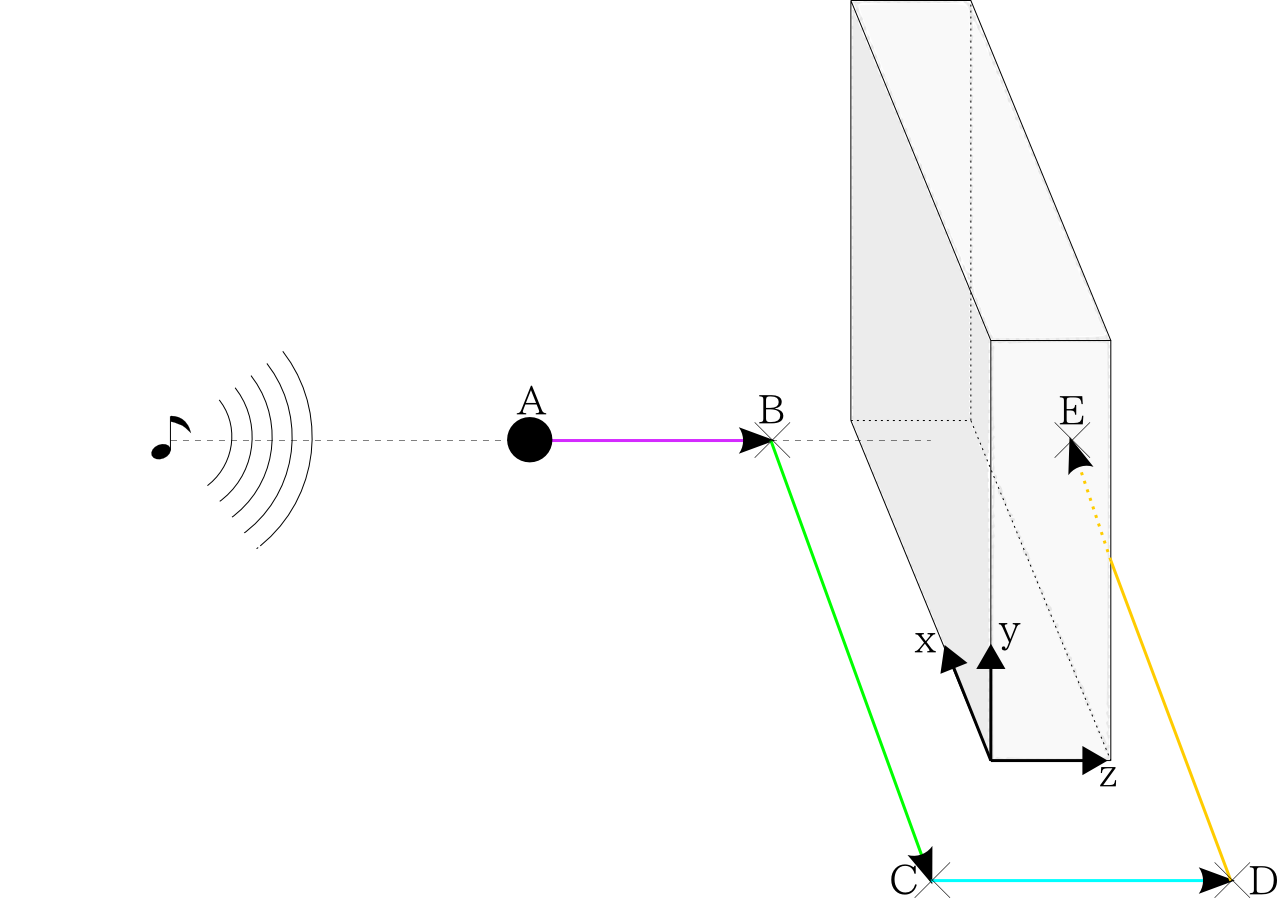
\includegraphics[clip,width=8.0cm]{./png/route.png}
    \caption{受音点の移動経路図}
    \label{fig:route}
  \end{center}
\end{figure}

\begin{figure}[H]
  \begin{center}
    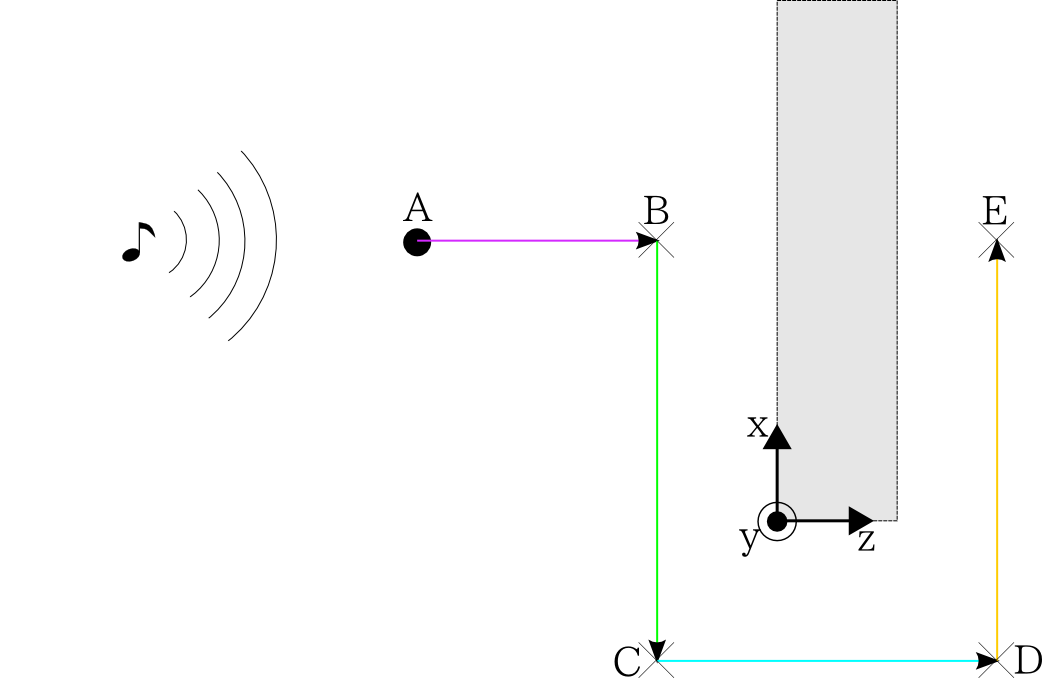
\includegraphics[clip,width=8.0cm]{./png/route_ue.png}
    \caption{受音点の移動経路をy軸正方向から見た図}
    \label{fig:route_ue}
  \end{center}
\end{figure}

\begin{figure}[H]
  \begin{center}
    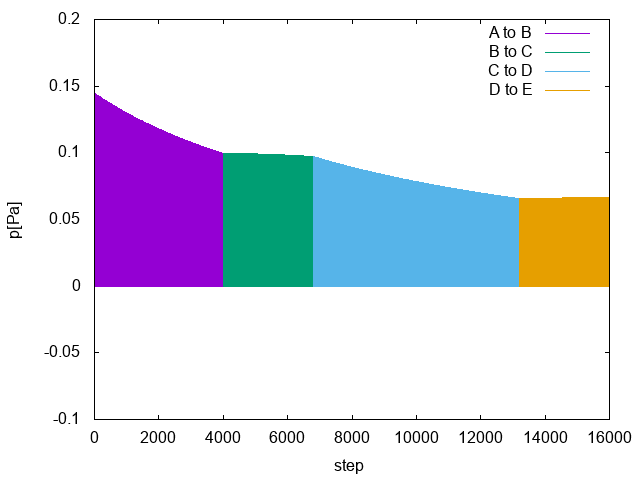
\includegraphics[clip,width=8.0cm]{./png/kyoukai_chokusetsu.png}
    \caption{移動しながら音源からの直接波のみを観測した場合の音圧}
    \label{fig:kyoukai_chokusetsu}
  \end{center}
\end{figure}\\

\begin{figure}[H]
  \begin{center}
    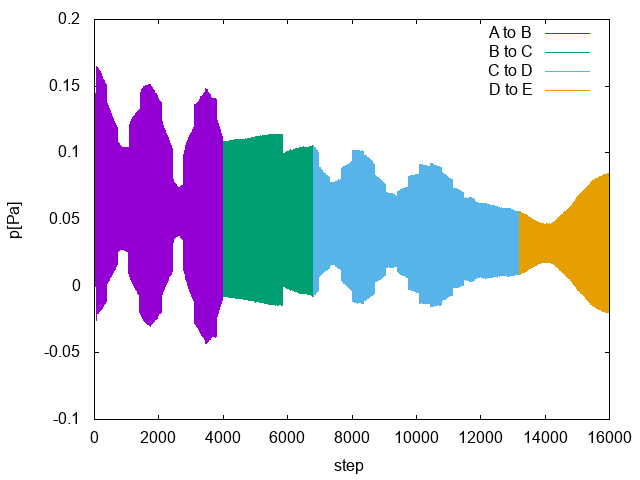
\includegraphics[clip,width=8.0cm]{./png/kyoukai_hansya.png}
    \caption{移動しながら音源からの散乱波のみを観測した場合の音圧}
    \label{fig:kyoukai_hansya}
  \end{center}
\end{figure}\\

\begin{figure}[H]
  \begin{center}
    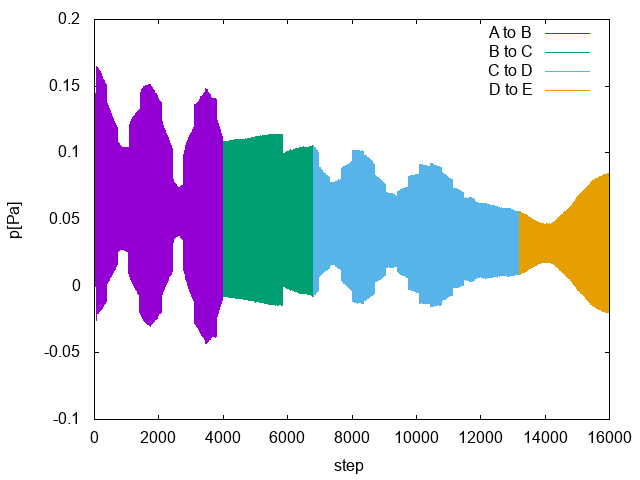
\includegraphics[clip,width=8.0cm]{./png/kyoukai_all.png}
    \caption{移動しながら音源から音圧を観測した場合の音圧}
    \label{fig:kyoukai_all}
  \end{center}
\end{figure}\\

%画面上のUIの説明をあとで追加



% フローチャート序論この研究をやります.
% 研究背景.適用こんなことやりまして、
% 結果を乗せる
% りあるたいむかちょうかにちかづいた
% 結論リアルタイムにどれだけ近づきました
% ホワイトボードの移動した奇跡と移動した結果の波形の画像をはっつける
\section{結論}
本論文は音圧を積分方程式法を近似することによる移動する受音点でのリアルタイム可聴化が目的である.
しかしながら,作成したシステムでは実行中に求める速度と比較し,大きな遅延が生じた.
\ref{問題設定}節で行った実行環境下では要求実行時間2[sec]に対し,およそ10[sec]かかった.
内点計算を各時間ステップ毎に実行するが,内点計算に要する時間が時間刻み幅$1.25 \times 10^{-4}$[sec]
以内に終了していないことが主な問題である.本システムでは内点計算の終了を待ち,
その後次ステップの計算を開始するよう設計されているために遅延が発生したと思われる.
また,受音点が3次元空間上を自由に動くことが可能であるため,画面の再描画も遅延の原因の一つである\par
今後の課題としては,リアルタイムでの処理に対応すべく並列計算等で高速化したい.

\clearpage
%%% 謝辞 %%%%%%%%%%%%%%%%%%%%%%%%%%%%%%%%%%%%%%%%%%%%%%%%%%%%%%%%%%%%%%%%%%%%%%%%
\acknowledgment
本研究に取り組むにあたって助言をいただいた吉川仁准教授に深く感謝する.

%%% 参考文献 %%%%%%%%%%%%%%%%%%%%%%%%%%%%%%%%%%%%%%%%%%%%%%%%%%%%%%%%%%%%%%%%%%%%
\addcontentsline{toc}{section}{\refname} % 目次に参考文献を追加する.
                                         % chapter使用時は削除すること.
\begin{thebibliography}{10}
\bibitem{vrsound}
田近伸二; 樫山和男; 志村正幸. VR 技術を用いた対話型道路交通騒音評価システムの構築. 応用力学論文集, 土木学会, 2010, 13: 231-240.
\bibitem{unity}
Unityの教科書 Unity 2017完全対応版 2D&3Dスマートフォンゲーム入門講座 (Entertainment&IDEA)
\end{thebibliography}


%%% BibTeX 等を用いる場合は,上の thebibliography 環境を消してここに該当コードを
%%% 挿入すること.
%% \bibliographystyle{...}
%% \bibliography{...}

%%% 付録 %%%%%%%%%%%%%%%%%%%%%%%%%%%%%%%%%%%%%%%%%%%%%%%%%%%%%%%%%%%%%%%%%%%%%%%%
%%% 付録は不要ならば削除してよい.
\appendix

\section{意味のない付録}
これは意味のない付録です.これは意味のない引用です\cite{polya1945}.

\begin{table}[htbp]
  \caption{これは意味のない表です.}
  \centering
  \begin{tabular}{c|cc}
      &  A  &  B \\
    \hline
    C &  70 & 80 \\
    D & 100 &  0
  \end{tabular}
\end{table}

%%% 本文ここまで %%%%%%%%%%%%%%%%%%%%%%%%%%%%%%%%%%%%%%%%%%%%%%%%%%%%%%%%%%%%%%%%
\fi
\ifoutputcover
\cleardoublepage
%%% 表紙,背表紙,提出用摘要 %%%%%%%%%%%%%%%%%%%%%%%%%%%%%%%%%%%%%%%%%%%%%%%%%%%%
\makecover                      % 表紙
\makespine[\numberofspines]     % 背表紙
\fi
\ifoutputabstractforsubmission
\makeabstractforsubmission      % 提出用摘要
\fi
\end{document}
